% ----------------------------------------------------
% Design
% ----------------------------------------------------
%\documentclass[class=report,11pt,crop=false]{standalone}
%% Page geometry
\usepackage[a4paper,margin=20mm,top=25mm,bottom=25mm]{geometry}

% Font choice
\usepackage{lmodern}

% Use IEEE bibliography style
\bibliographystyle{IEEEtran}

% Line spacing
\usepackage{setspace}
\setstretch{1.20}

% Allows us to create dummy text
\usepackage{lipsum}

% Ensure UTF8 encoding
\usepackage[utf8]{inputenc}

% Language standard (not too important)
\usepackage[english]{babel}

% Skip a line in between paragraphs
\usepackage{parskip}

% For the creation of dummy text
\usepackage{blindtext}

% Math
\usepackage{amsmath}

% Header & Footer stuff
\usepackage{fancyhdr}
\pagestyle{fancy}
\fancyhead{}
\fancyhead[R]{\nouppercase{\rightmark}}
\fancyfoot{}
\fancyfoot[C]{\thepage}
\renewcommand{\headrulewidth}{0.0pt}
\renewcommand{\footrulewidth}{0.0pt}
\setlength{\headheight}{13.6pt}

% Epigraphs
\usepackage{epigraph}
\setlength\epigraphrule{0pt}
\setlength{\epigraphwidth}{0.65\textwidth}

% Colour
\usepackage{color}
\usepackage[dvipsnames]{xcolor}

% Hyperlinks & References
\usepackage{hyperref}
\definecolor{linkColour}{RGB}{77,71,179}
\hypersetup{
    colorlinks=true,
    linkcolor=linkColour,
    filecolor=linkColour,
    urlcolor=linkColour,
    citecolor=linkColour,
}
\urlstyle{same}

% Automatically correct front-side quotes
\usepackage[autostyle=false, style=ukenglish]{csquotes}
\MakeOuterQuote{"}

% Graphics
\usepackage{graphicx}
\graphicspath{{Images/}{../Images/}}
\usepackage{makecell}
\usepackage{transparent}

% SI units
\usepackage{siunitx}

% Microtype goodness
\usepackage{microtype}

% Listings
\usepackage[T1]{fontenc}
\usepackage{listings}
\usepackage[scaled=0.8]{DejaVuSansMono}

% Custom colours for listings
\definecolor{backgroundColour}{RGB}{250,250,250}
\definecolor{commentColour}{RGB}{73, 175, 102}
\definecolor{identifierColour}{RGB}{196, 19, 66}
\definecolor{stringColour}{RGB}{252, 156, 30}
\definecolor{keywordColour}{RGB}{50, 38, 224}
\definecolor{lineNumbersColour}{RGB}{127,127,127}
\lstset{
  language=Matlab,
  captionpos=b,
  aboveskip=15pt,belowskip=10pt,
  backgroundcolor=\color{backgroundColour},
  basicstyle=\ttfamily,%\footnotesize,        % the size of the fonts that are used for the code
  breakatwhitespace=false,         % sets if automatic breaks should only happen at whitespace
  breaklines=true,                 % sets automatic line breaking
  postbreak=\mbox{\textcolor{red}{$\hookrightarrow$}\space},
  commentstyle=\color{commentColour},    % comment style
  identifierstyle=\color{identifierColour},
  stringstyle=\color{stringColour},
   keywordstyle=\color{keywordColour},       % keyword style
  %escapeinside={\%*}{*)},          % if you want to add LaTeX within your code
  extendedchars=true,              % lets you use non-ASCII characters; for 8-bits encodings only, does not work with UTF-8
  frame=single,	                   % adds a frame around the code
  keepspaces=true,                 % keeps spaces in text, useful for keeping indentation of code (possibly needs columns=flexible)
  morekeywords={*,...},            % if you want to add more keywords to the set
  numbers=left,                    % where to put the line-numbers; possible values are (none, left, right)
  numbersep=5pt,                   % how far the line-numbers are from the code
  numberstyle=\tiny\color{lineNumbersColour}, % the style that is used for the line-numbers
  rulecolor=\color{black},         % if not set, the frame-color may be changed on line-breaks within not-black text (e.g. comments (green here))
  showspaces=false,                % show spaces everywhere adding particular underscores; it overrides 'showstringspaces'
  showstringspaces=false,          % underline spaces within strings only
  showtabs=false,                  % show tabs within strings adding particular underscores
  stepnumber=1,                    % the step between two line-numbers. If it's 1, each line will be numbered
  tabsize=2,	                   % sets default tabsize to 2 spaces
  %title=\lstname                   % show the filename of files included with \lstinputlisting; also try caption instead of title
}

% Caption stuff
\usepackage[hypcap=true, justification=centering]{caption}
\usepackage{subcaption}

% Glossary package
% \usepackage[acronym]{glossaries}
\usepackage{glossaries-extra}
\setabbreviationstyle[acronym]{long-short}

% For Proofs & Theorems
\usepackage{amsthm}

% Maths symbols
\usepackage{amssymb}
\usepackage{mathrsfs}
\usepackage{mathtools}

% For algorithms
\usepackage[]{algorithm2e}

% Spacing stuff
\setlength{\abovecaptionskip}{5pt plus 3pt minus 2pt}
\setlength{\belowcaptionskip}{5pt plus 3pt minus 2pt}
\setlength{\textfloatsep}{10pt plus 3pt minus 2pt}
\setlength{\intextsep}{15pt plus 3pt minus 2pt}

% For aligning footnotes at bottom of page, instead of hugging text
\usepackage[bottom]{footmisc}

% Add LoF, Bib, etc. to ToC
\usepackage[nottoc]{tocbibind}

% SI
\usepackage{siunitx}

% For removing some whitespace in Chapter headings etc
\usepackage{etoolbox}
\makeatletter
\patchcmd{\@makechapterhead}{\vspace*{50\p@}}{\vspace*{-10pt}}{}{}%
\patchcmd{\@makeschapterhead}{\vspace*{50\p@}}{\vspace*{-10pt}}{}{}%
\makeatother
%
\newacronym{radar}{RADAR}{Radio Detection and Ranging}

%\begin{document}
% ----------------------------------------------------
\chapter{System Design \label{ch:design}}\label{sec:SysD}
%\epigraph{Oh, to see without my eyes.}%
%    {\emph{---Sufjan Stevens}}
\vspace{0.5cm}
% ----------------------------------------------------

    \begin{figure}[H]
    \centering
    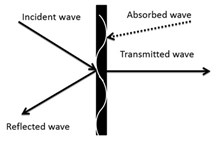
\includegraphics[width=0.4\linewidth]{Figures/chp3_incident_wave.png}
    \caption{Wave incident at a dielectric boundary.}
    \label{fig:chp3_incident_wave}
    \end{figure}
    
Figure \ref{fig:chp3_incident_wave} above shows the different waves present when a wave is incident at a dielectric boundary. The hypothesis for the proposed system in section \ref{sec:objectives} is that the absorbed wave induces currents on the reflector array. Then these induced currents cause the reflector array elements to re-radiate the majority of the absorbed wave again. If it is assumed that this is true, the goal is to then encode the re-radiated wave with a phase difference by changing the termination of the reflector array elements from and open to a short circuit and back. To verify if this is possible an antenna is designed and 3 different versions of the designed antenna is manufactured. Each version only changes load connected to the antenna.

\section{Simulation based investigation}
The initial investigation was planned to be simulation based and due do the ease of Farfield simulations in FEKO, the investigation started in FEKO. However, after many complications two major changes were made. Firstly, the final investigation changed from simulation based to physical measurements due to the required simulation model becoming too complex to implement in FEKO. The Planar wave source is not bounded with a specific beamwidth and the Farfield monitors do not measure the S21 parameter.

Secondly, the antenna design moved from FEKO to CST Studio, due to the complex microstrip design required. The stack-up changed to asymmetrical stack-up, which required an X-band via as well.

This section documents the obstacles and restrictions faced when trying to complete the investigation based only on simulations.

\subsection{Antenna design and ports in FEKO}
FEKO provides different port setups, including wire, edge and waveguide ports. It is not clear which port is ideal for the antenna model. The waveguide port requires a waveguide structure in the model to be able to use. The antenna model seen in figure \ref{fig:chp3_patch_wire_port} below does not have a waveguide structure. The remaining port options are wire and edge ports.

    \begin{figure}[H]
    \centering
    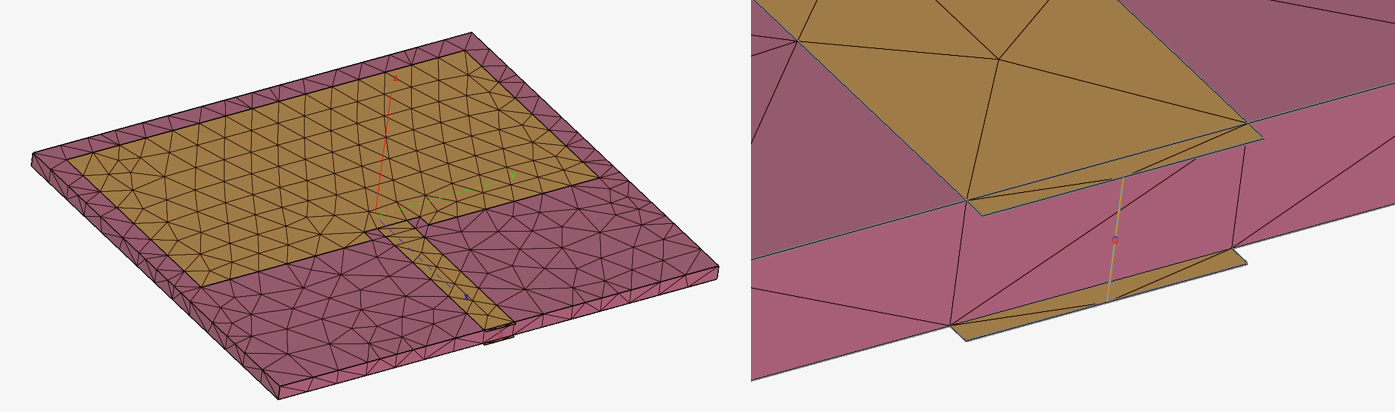
\includegraphics[width=0.7\linewidth]{Figures/chp3_patch_wire_port.png}
    \caption{Patch antenna model in FEKO using a wire port.}
    \label{fig:chp3_patch_wire_port}
    \end{figure}

The figure \ref{fig:chp3_patch_wire_port} above uses a wire port with a voltage source. Using the wire port requires the 50$\Omega$ trace to extend past the edge of the board and then assigning a wire radius to the wire port. There is no clear documentation for how to define the distance the trace should extend or how to determine the required wire radius. Figure \ref{fig:chp3_patch_wire_port_S11} shows the return loss of -12dB at a center frequency of 9.5GHz.

    \begin{figure}[H]
    \centering
    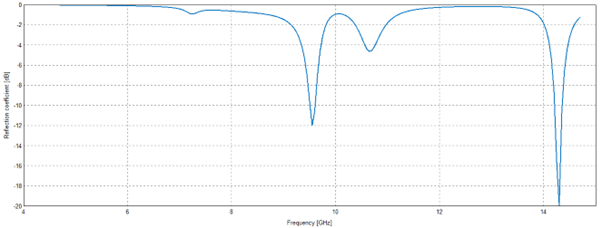
\includegraphics[width=0.95\linewidth]{Figures/chp3_patch_wire_port_S11.png}
    \caption{Return loss of the patch in figure \ref{fig:chp3_patch_wire_port}}
    \label{fig:chp3_patch_wire_port_S11}
    \end{figure}

The figure \ref{fig:chp3_patch_wire_port_pattern} show the Farfield pattern at the center frequency of the antenna. Since gain of 5.9dBi is observed, it can be concluded that the wire port is setup correctly, however the frequency response at frequencies greater than 14GHz seem inaccurate.

    \begin{figure}[H]
    \centering
    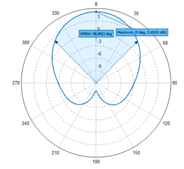
\includegraphics[width=0.4\linewidth]{Figures/chp3_patch_wire_port_pattern.png}
    \caption{Antenna pattern of the patch in figure \ref{fig:chp3_patch_wire_port}}
    \label{fig:chp3_patch_wire_port_pattern}
    \end{figure}

The figure \ref{fig:chp3_patch_edge_port} uses an edge port with a voltage source. Using the edge port also requires the 50$\Omega$ trace to extend past the edge of the board however no wire radius is required. Therefor removing one of the uncertainties. Figure \ref{fig:chp3_patch_edge_port_S11} shows the return loss of -24dB at a center frequency of 9.5GHz, which is an significant improvement over the wire port model. The frequency response at frequencies greater than 14GHz seem more realistic. From these results it is assumed that is edge port feed is more accurate for this model, however the only way to verify is to build and test the antenna.

    \begin{figure}[H]
    \centering
    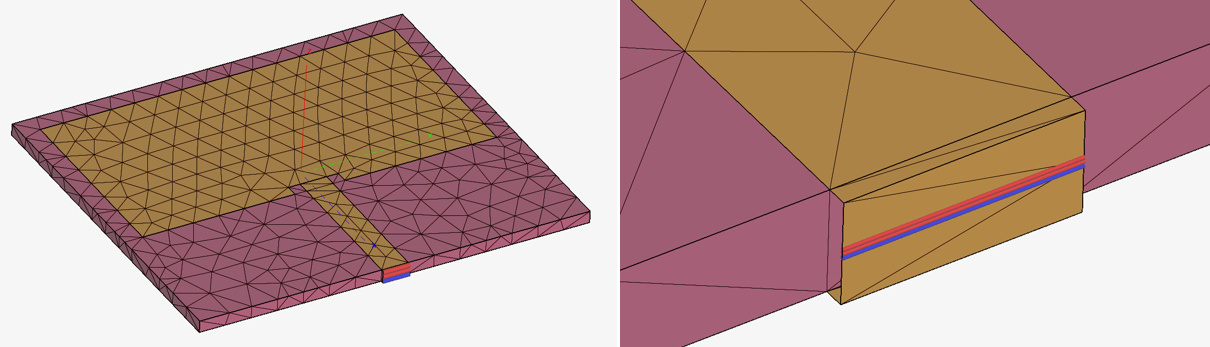
\includegraphics[width=0.7\linewidth]{Figures/chp3_patch_edge_port.png}
    \caption{Patch antenna model in FEKO using a edge port.}
    \label{fig:chp3_patch_edge_port}
    \end{figure}

    \begin{figure}[H]
    \centering
    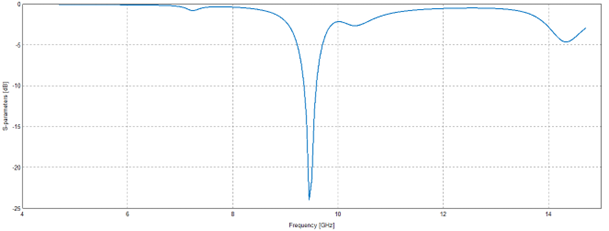
\includegraphics[width=0.95\linewidth]{Figures/chp3_patch_edge_port_S11.png}
    \caption{Return loss of the patch in figure \ref{fig:chp3_patch_edge_port}}
    \label{fig:chp3_patch_edge_port_S11}
    \end{figure}

\subsection{{Phase \& Planar wave \& Dipole monitor}}
The next step is to radiate the patch antenna (AUT) with a RF signal and measure the phase of the reflected signal. The approach was to use FEKO’s planar wave source to radiate the AUT and then place a dipole in the Farfield with a wire port. To connect a load to the antenna, a port is required on the antenna as well. This load is varied from 0$\Omega$ to 50$\Omega$ to 10M$\Omega$.

    \begin{figure}[H]
    \centering
    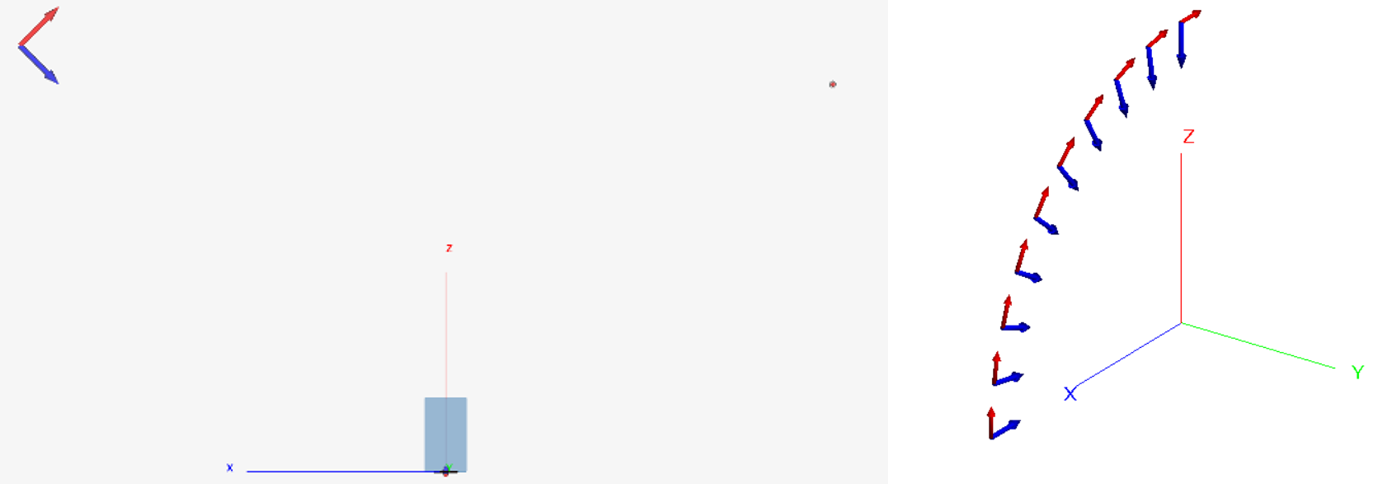
\includegraphics[width=0.8\linewidth]{Figures/chp3_simulation_setup.png}
    \caption{FEKO simulation setup using a dipole with a wire port as the monitor.}
    \label{fig:chp3_simulation_setup}
    \end{figure}

The figure \ref{fig:chp3_simulation_setup} show the planar wave source in the top left corner, the AUT in the middle and the dipole in the top right corner. Figure \ref{fig:chp3_simulation_setup} shows the planar wave source swept from 0° to 90°. One problem with this approach is that the planar wave source is not bounded and radiates the dipole as well, see figure \ref{fig:chp3_planar_source_unbounded}. The dipole is omnidirectional and will absorb the planar wave. One solution to this is to use an antenna to radiate the AUT, however the simulation model becomes exponentially more complex to run.

    \begin{figure}[H]
    \centering
    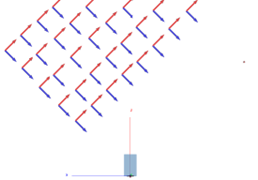
\includegraphics[width=0.4\linewidth]{Figures/chp3_planar_source_unbounded.png}
    \caption{Visual representation of the unbounded planar wave source in FEKO.}
    \label{fig:chp3_planar_source_unbounded}
    \end{figure}

An alternative approach is to use the Farfield result to measure the theoretical received phase if an receiver where to be place in the Farfield. Figure \ref{fig:chp3_simulation_farfield_setup} below shows the planar wave source swept from 0° to 90° in red and the Farfield monitor setup from 90° to 180°. With this approach FEKO already calibrates out the phase from the planar wave source. This is verified by removing the AUT and observing a constant 0° phase in the Farfield E-field phase.

    \begin{figure}[H]
    \centering
    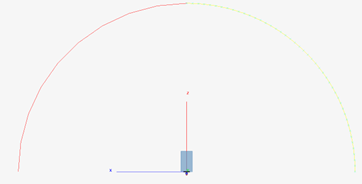
\includegraphics[width=0.65\linewidth]{Figures/chp3_simulation_farfield_setup.png}
    \caption{FEKO simulation setup using a farfield monitor.}
    \label{fig:chp3_simulation_farfield_setup}
    \end{figure}

Part of the simulated investigation is to see if the feed length changes the phase response. Using the model in figure \ref{fig:chp3_patch_coax_port} and changing the feed length would also change the ground plane size. Changing the ground plane size or the physical AUT structure that the planar wave radiates will change the phase response due a larger reflective surface. However, to observe the phase change due to the absorbed wave propagating in the feed, the physical AUT structure that the planar wave radiates must remain fixed. One way to achieve this is to use a trough hole feed and a coaxial structure behind the antenna that can change in length. This approach has a similar problem as seen in figure \ref{fig:chp3_planar_source_unbounded}, where the planar wave will reflect off the coaxial cable to the planar wave not being bounded to the top of the AUT.

    \begin{figure}[H]
    \centering
    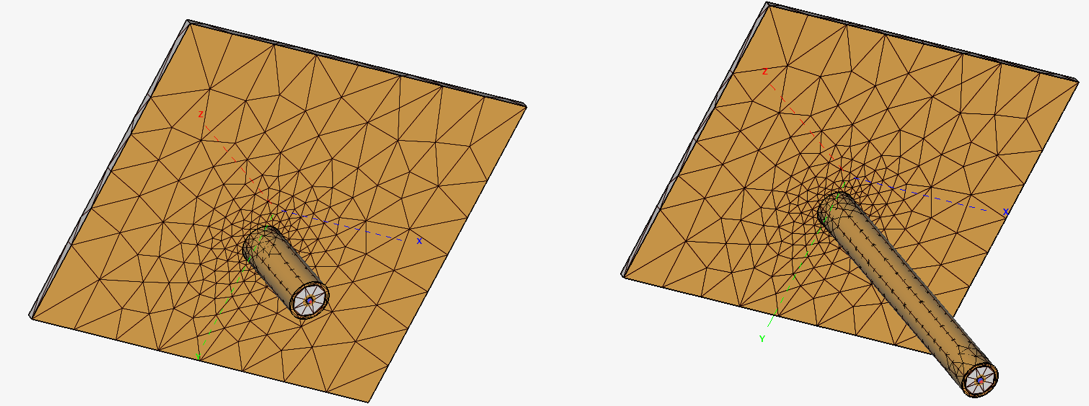
\includegraphics[width=0.65\linewidth]{Figures/chp3_patch_coax_port.png}
    \caption{Patch antenna model with a variable coaxial cable}
    \label{fig:chp3_patch_coax_port}
    \end{figure}

\subsection{Coax \& CPW}
Simulating the model in figure \ref{fig:chp3_patch_coax_port} results in a extremely poor return loss. The port type was changed to verify that the port setup is not the source of the poor return loss, however the return loss remained worse than -12dB for all port types used. After many failed attempts of trying to improve the match a very simple 50$\Omega$ microstrip model was created to verify that that simulates correctly. Figure \ref{fig:chp3_microstrip_edge_port_combined} show the microstrip model along with the simulation results. The result is indeed a 50$\Omega$ matched microstrip.

    \begin{figure}[H]
    \centering
    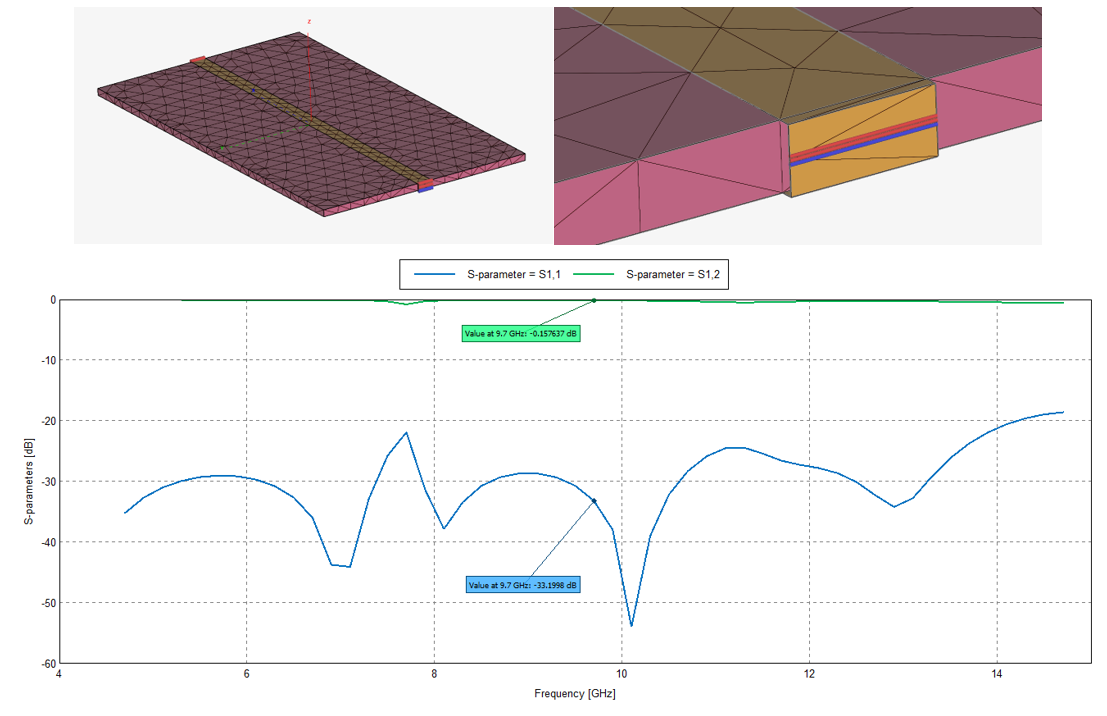
\includegraphics[width=0.8\linewidth]{Figures/chp3_microstrip_edge_port_combined.png}
    \caption{Microstrip model in FEKO using a edge port along with the frequency response.}
    \label{fig:chp3_microstrip_edge_port_combined}
    \end{figure}

Next a simple 50$\Omega$ CPW model was created to verify that that simulates correctly. Figure \ref{fig:chp3_CPW_edge_port_combined} below show the CPW model along with the simulation results. The return loss at X-Band is very poor.

    \begin{figure}[H]
    \centering
    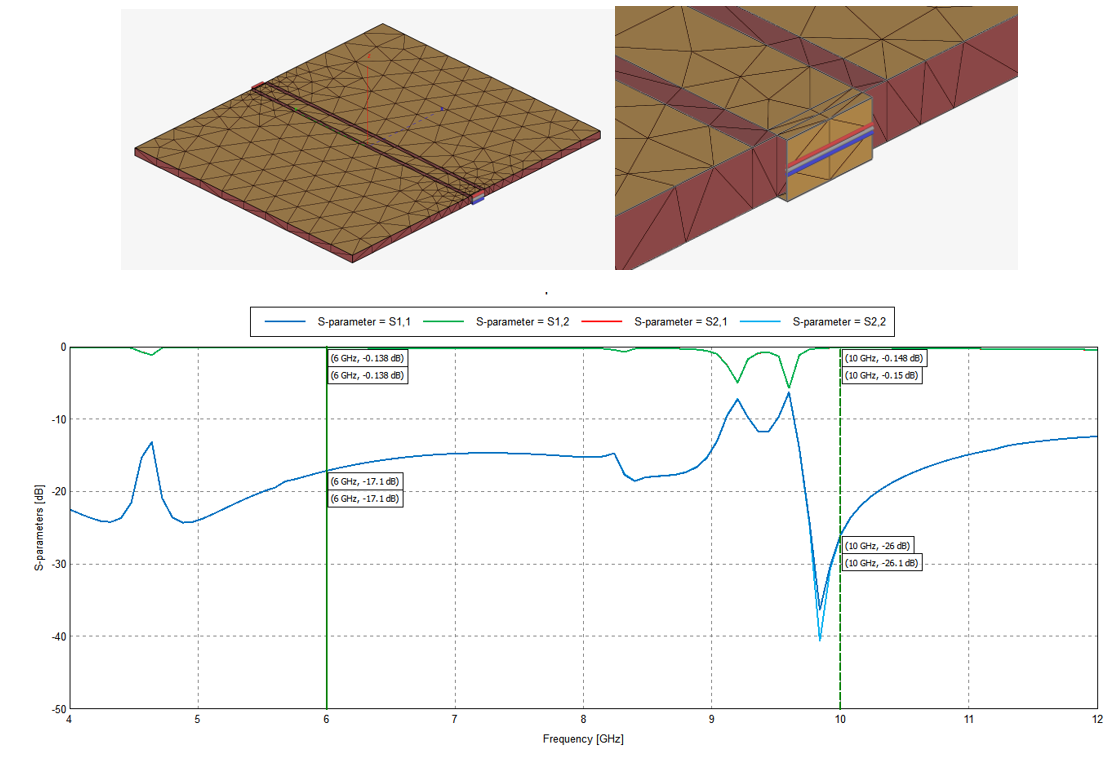
\includegraphics[width=0.8\linewidth]{Figures/chp3_CPW_edge_port_combined.png}
    \caption{CPW model in FEKO using a edge port along with the frequency response.}
    \label{fig:chp3_CPW_edge_port_combined}
    \end{figure}

Assuming that the edge port is not correct due to the port not making contact with the ground planes either side of the trace, Altair support was contacted for assistance. The model was revised base based on the comments from Altair and the model is seen in figure \ref{fig:chp3_CPW_altair_port}. The port now involves a larger copper plane that touches the bottom ground layer, the trace and the ground plane on both sides of the trace. Furthermore, a small section of the PCB needs to be cut away since the edge port cannot be place on the edge of a dielectric medium.

    \begin{figure}[H]
    \centering
    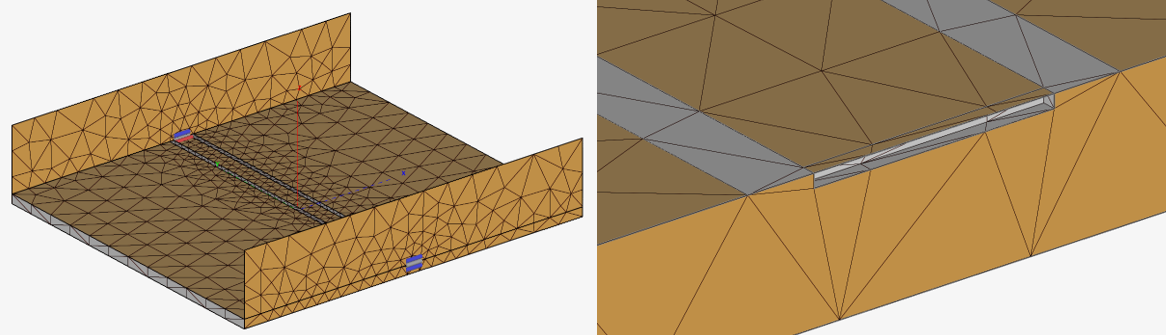
\includegraphics[width=0.6\linewidth]{Figures/chp3_CPW_altair_port.png}
    \caption{CPW model in FEKO using the supplied port from Altair support.}
    \label{fig:chp3_CPW_altair_port}
    \end{figure}

Figure \ref{fig:chp3_CPW_altair_port_results} show the wide band response of the CPW model and a good match is observed at 7.2GHz, however a very poor match is observed at X-band. This exact CPW structure has successfully been used in radar design in the past. Figure \ref{fig:chp3_CPW_altair_port_results_zoom} shows a zoom-in frequency response.  That specific radar operated form 9.2 to 9.75GHz with very little losses. Knowing this the results still seem inaccurate.

    \begin{figure}[H]
    \centering
    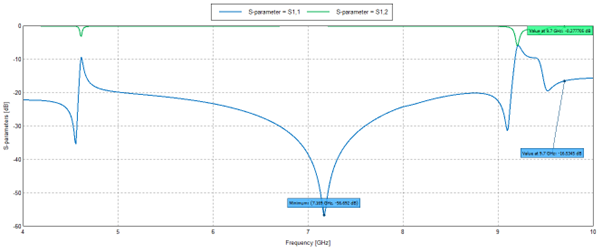
\includegraphics[width=0.9\linewidth]{Figures/chp3_CPW_altair_port_results.png}
    \caption{Frequency response of the CPW model in figure \ref{fig:chp3_CPW_altair_port}}
    \label{fig:chp3_CPW_altair_port_results}
    \end{figure}

    \begin{figure}[H]
    \centering
    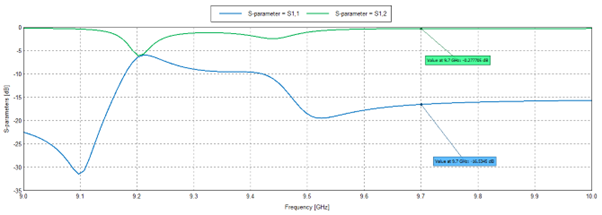
\includegraphics[width=0.9\linewidth]{Figures/chp3_CPW_altair_port_results_zoom.png}
    \caption{X-band frequency response of the CPW model in figure \ref{fig:chp3_CPW_altair_port}}
    \label{fig:chp3_CPW_altair_port_results_zoom}
    \end{figure}

\subsection{CST Studio}
The decision was made to move to designing the antenna in CST Studio and manufacturing the antenna to continue the investigation. 

Firstly, the very same simple 50$\Omega$ CPW model was created to verify that that simulates correctly. Figure \ref{fig:chp3_CPW_CST_waveguide_port} show the CPW model in CST Studio. Figure \ref{fig:chp3_CPW_CST_mesh}. The result is indeed a 50$\Omega$ matched microstrip, see figure \ref{fig:chp3_CPW_CST_impedance}.

    \begin{figure}[H]
    \centering
    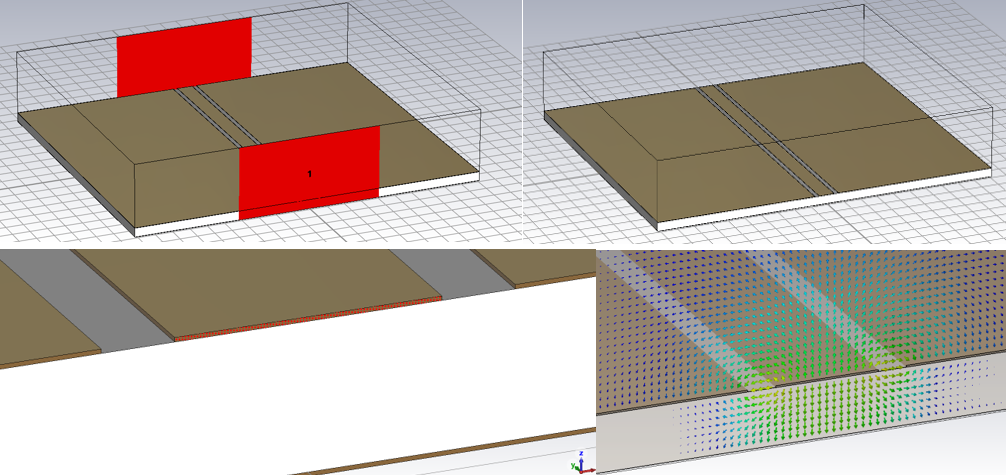
\includegraphics[width=0.7\linewidth]{Figures/chp3_CPW_CST_waveguide_port.png}
    \caption{CPW model in CST using waveguide ports.}
    \label{fig:chp3_CPW_CST_waveguide_port}
    \end{figure}

    \begin{figure}[H]
    \centering
    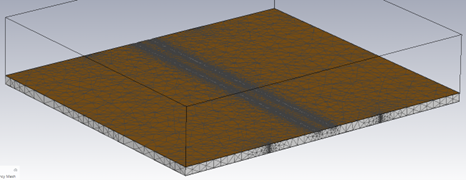
\includegraphics[width=0.5\linewidth]{Figures/chp3_CPW_CST_mesh.png}
    \caption{Meshed CPW model in CST.}
    \label{fig:chp3_CPW_CST_mesh}
    \end{figure}

    \begin{figure}[H]
    \centering
    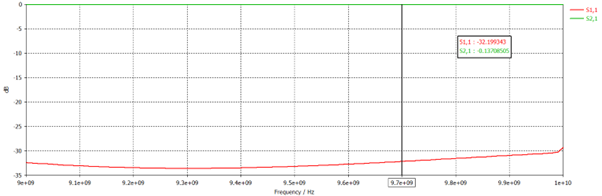
\includegraphics[width=0.9\linewidth]{Figures/chp3_CPW_CST_results_zoom.png}
    \caption{X-band frequency response of the CPW model in figure \ref{fig:chp3_CPW_CST_waveguide_port}}
    \label{fig:chp3_CPW_CST_results_zoom}
    \end{figure}

    \begin{figure}[H]
    \centering
    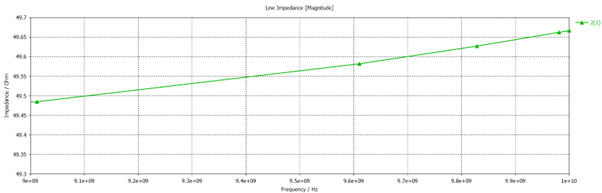
\includegraphics[width=0.9\linewidth]{Figures/chp3_CPW_CST_impedance.png}
    \caption{Line impedance of the CPW model in figure \ref{fig:chp3_CPW_CST_waveguide_port}.}
    \label{fig:chp3_CPW_CST_impedance}
    \end{figure}
    
\section{Antenna Detail Design}
\subsection{Center frequency}\label{sec:centerFreq}
The antenna is chosen to be a X-Band antenna as this results in a very small antenna element and therefore a relatively small reflector array if these antennas where to be used for future testing. Due to the antenna element being small, the far-field distance remains short enough to be able to test in the laboratory with a VNA. The center frequency is chosen as 9.7GHz as this is the center frequency of an existing radar and could be used to test the final proposed system in the future. 
    \[\lambda=\frac{c_0}{f_c}=\frac{c_0}{\left(9.7GHz\right)}=30.91\ mm\]

\subsection{PCB Stack-up}
A FR-4 substrate will be very lossy at X-band \cite{Substrate}. Rogers RO4003C is common substrate used for X-band applications as the Dissipation Factor (\(tan\delta\)) or Loss Tangent (\(Df\)) is significantly lower that FR-4.

    \begin{table}[H]
    \centering
    \caption{Dielectric comparison.}
    \begin{tabular}{|l|l|l|} 
    \hline
    \textbf{Parameter} & \textbf{FR-4}    & \textbf{RO4003C}  \\ 
    \hline
    Dk                 & 4.35 @ 500MHz    & 3.38 @ 10GHz      \\ 
    \hline
    Df                 & 0.017 @ 500MHz & 0.0027 @10GHz     \\
    \hline
    \end{tabular}
    \label{tab:PVresults}
    \end{table}

To mask the feed of the individual antenna elements the feed must be on the back of the PCB with a solid ground plane separating the feed and the patch. Therefor a minimum of 3 layers is required. The final stack-up is seen figure \ref{fig:chp3_stackup}

    \begin{figure}[H]
    \centering
    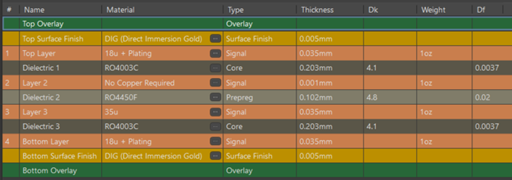
\includegraphics[width=0.8\linewidth]{Figures/chp3_stackup.png}
    \caption{PCB stackup used for the antenna design.}
    \label{fig:chp3_stackup}
    \end{figure}

If the third layer is used for the ground plane, then the second layer is not required. By removing the copper from the second layer the substrate height increases as the substrate now consists of both the RO4450F and RO4003C. This increase in substrate height will increase the bandwidth of the antenna due to an increase in fringing fields \cite{Fringing}.

Rogers provides a Microwave Impedance Calculator tool to calculate the dielectric properties for a given stack-up and frequency. The composite dielectric constant at 9.7GHz is calculated as 3.78 using the tool, see figure \ref{fig:chp3_MWI}. 

    \begin{figure}[H]
    \centering
    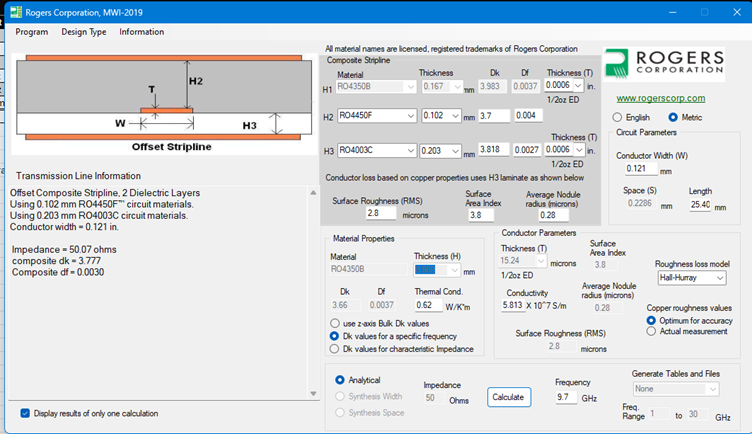
\includegraphics[width=0.8\linewidth]{Figures/chp3_MWI.png}
    \caption{Roger Corporation's Microwave Impedance Calculator.}
    \label{fig:chp3_MWI}
    \end{figure}

\subsection{Patch Dimensions}
The patch length for a half wave patch antenna is calculated as follows \cite{patchDimensions}. This is an approximation and will need to be tuned during simulations.
    \[f_c\approx\frac{c_0}{2L\sqrt{\varepsilon_r}}\]
    \[L\approx\frac{c_0}{2f_c\sqrt{\varepsilon_r}}=\frac{c_0}{2\left(9.7GHz\right)\sqrt{3.78}}=7.95mm\]

The bandwidth of the antenna is determined by the width of the patch. The radar mentioned in section \ref{sec:centerFreq} has a 150MHz bandwidth and the antenna is designed to match the radar’s bandwidth. The patch width is calculated as follows. This is an approximation and will need to be tuned during simulations.
    \[B_{-10dB}=3.77f_c\ast\frac{\varepsilon_r-1}{\varepsilon_r^2}\ast\frac{W}{L}\ast\frac{t}{\lambda}\]
    \[W=\frac{\varepsilon_r^2\ast L\ast\lambda\ast B}{3.77\ast\left(\varepsilon_r-1\right)\ast t\ast f_c}\]
    \[W=\frac{\left(3.78\right)^2(7.95mm)(30.91mm)(150MHz)}{3.77\left(3.78-1\right)(0.305mm)(9.7GHz)}=16.98mm\]

The size of the ground plane width (\(W_g\)) must be sufficiently large that the fringing fields do not exceed the edges of the ground plane. Since fringing fields are proportional to the substrate height, the distance from the edge of the patch to the edge of the ground plane (\(\Delta _g\)) needs be significantly larger than the substrate thickness to ensure that fringing fields do not exceed the edges of the ground plane. \(\Delta _g\) is designed to be approximately 10 times larger than the substrate thickness (\(t\)).
    \[\Delta_g\gg\ t,\ \ \ \ \ \ \Delta_g\gg0.305mm\]
    \[\Delta_g\approx10\ast\ t\approx10(0.305mm)\approx3.05mm\]
    \[W_g=W+\Delta _g=16.98+3.05=20.03\approx 20mm\]

The ground plane length (\(L_g\)) needs to be large enough to fit the feed and an arbitrary length of 25mm is chosen but can be increase if needed when the feed is designed.
    \[L_g>L+\Delta_g\]
    \[L_g>11mm\]
    \[L_g\approx25mm\]

The final parameter needed for the initial simulation is 50$\Omega$ trace width. This is calculated again using the Microwave Impedance Calculator tool, but the \textit{Design Type} is changed to microstrip, and the dielectric constant is manually changed to the calculated composite dielectric constant. The 50$\Omega$ trace width as 0.681mm. 

    \begin{figure}[H]
    \centering
    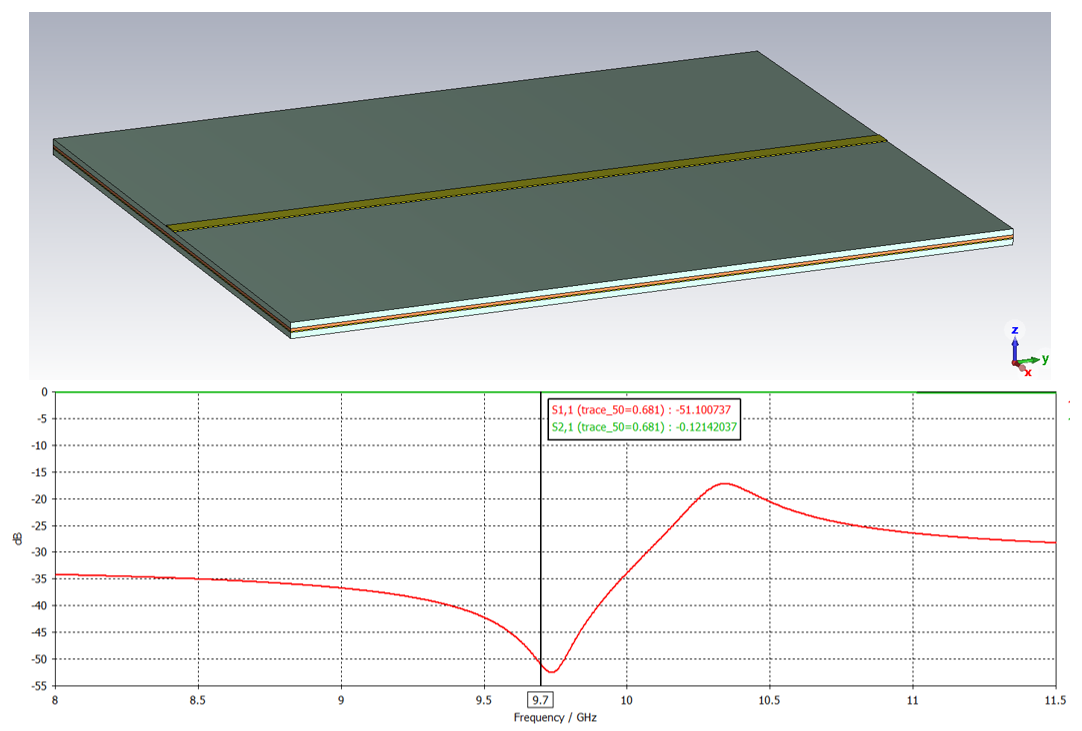
\includegraphics[width=0.9\linewidth]{Figures/chp3_CST_microstrip_combined.png}
    \caption{Microstrip model in CST with the frequency response.}
    \label{fig:chp3_CST_microstrip_combined}
    \end{figure}

Due past difficulty with simulation software, the 50$\Omega$ trace is simulated to verify the PCB model is setup correctly. Figure \ref{fig:chp3_CST_microstrip_combined} shows the model and simulated frequency response of the designed 50$\Omega$ trace at 9.7GHz. A 51.10dB return loss is seen at 9.7GHz. The loss over a 25mm trace is 0.12dB. This verifies the model and solver are setup correctly.

    \begin{figure}[H]
    \centering
    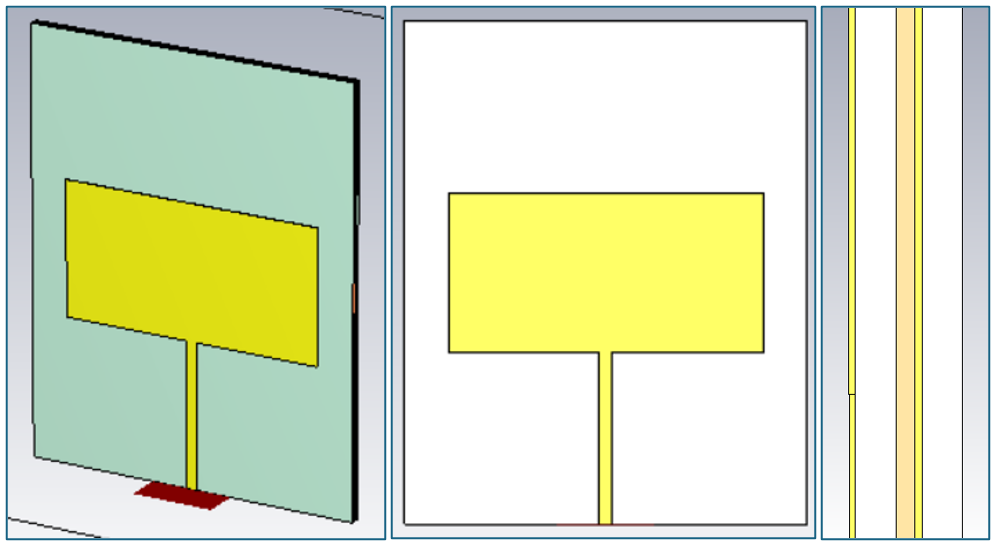
\includegraphics[width=0.5\linewidth]{Figures/chp3_CPW_patch.png}
    \caption{Patch antenna model in CST.}
    \label{fig:chp3_CPW_patch}
    \end{figure}

Figure \ref{fig:chp3_CPW_patch} shows the initial CST Studio model used to tune the patch length and width for the designed frequency and bandwidth. Figure ? below shows the results for the initial model without any parameter tuned. 

    \begin{figure}[H]
    \centering
    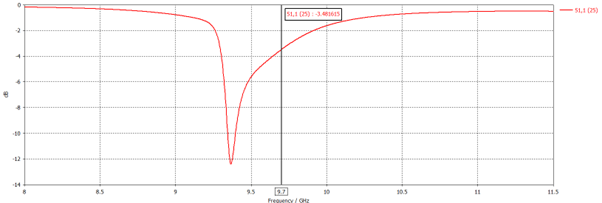
\includegraphics[width=0.9\linewidth]{Figures/chp3_CPW_patch_results.png}
    \caption{Frequency response of the patch antenna in figure \ref{fig:chp3_CPW_patch}.}
    \label{fig:chp3_CPW_patch_results}
    \end{figure}

It is observed that the center frequency is lower than the designed center frequency of 9.7GHz. The center frequency is inversely proportional to the wavelength and the wavelength is directly proportional to the dimension of the patch. Therefor the center frequency can be increased by decreasing the length of the patch, but since the width of the patch is also dependent on the length of the patch, both dimensions should slowly be decreased until the center frequency is equal to 9.7GHz. Figure \ref{fig:chp3_CPW_patch_sweep_results} shows the return loss for the tuning of the center frequency. 

    \begin{figure}[H]
    \centering
    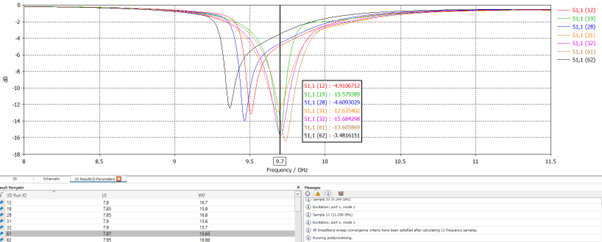
\includegraphics[width=0.95\linewidth]{Figures/chp3_CPW_patch_sweep_results.png}
    \caption{Parameter sweep results of the patch antenna in figure \ref{fig:chp3_CPW_patch}.}
    \label{fig:chp3_CPW_patch_sweep_results}
    \end{figure}

The final patch dimensions are
\[L=7.87mm\]
\[W=15.65mm\]

    \begin{figure}[H]
    \centering
    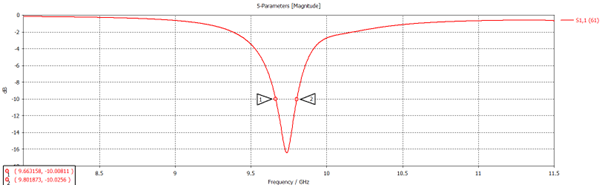
\includegraphics[width=0.95\linewidth]{Figures/chp3_CPW_patch_tuned_results.png}
    \caption{Return loss of the patch antenna before designing the feed inset.}
    \label{fig:chp3_CPW_patch_tuned_results}
    \end{figure}

Figure \ref{fig:chp3_CPW_patch_tuned_results} above shows the return loss of the single patch before the feed is designed, it is seen that the -10dB bandwidth (\(B_{-10dB}\)) is slightly lower than designed value of 150MHz. It is acceptable at this stage of the design for two reasons. Firstly, the radar bandwidth is measured from the -3dB point and the antenna bandwidth is measured from the -10dB point. Secondly the bandwidth will also change with the antenna feed design.
    \[B_{-10dB}=138.72\ MHz\]

\subsection{Feed inset}
The first step to match the patch to a 50$\Omega$ system is to design a feed inset. The theoretical impedance at the edge of the patch (\(Z_A\)) is calculated as
    \[Z_A=90\frac{\varepsilon_r^2}{\varepsilon_r-1}\left(\frac{L}{W}\right)^2\]
    \[Z_A=90\frac{({3.78)}^2}{(3.78)-1}\left(\frac{7.87mm}{15.65mm}\right)^2=117\ \Omega\]

The impedance decreases as the feed inset moves towards the center of the patch, where the impedance will be 0$\Omega$. Since the edge impedance (\(Z_A\)) is high then the desired 50$\Omega$, the inset is swept from the edge to the center of the patch.

    \begin{figure}[H]
    \centering
    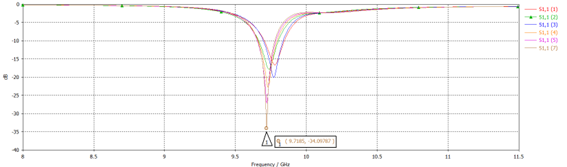
\includegraphics[width=0.95\linewidth]{Figures/chp3_CPW_patch_inset_sweep_results.png}
    \caption{Parameter sweep results of the patch antenna's feed inset.}
    \label{fig:chp3_CPW_patch_inset_sweep_results}
    \end{figure}

Figure \ref{fig:chp3_CPW_patch_inset_sweep_results} above shows the Return Loss of the patch as the inset in increased in steps of 0.1mm. The best performance is achieved with an inset depth of 0.6mm and the model is seen in figure \ref{fig:chp3_CPW_patch_inset} below. It is observed that the return loss improves by 17.5dB.

    \begin{figure}[H]
    \centering
    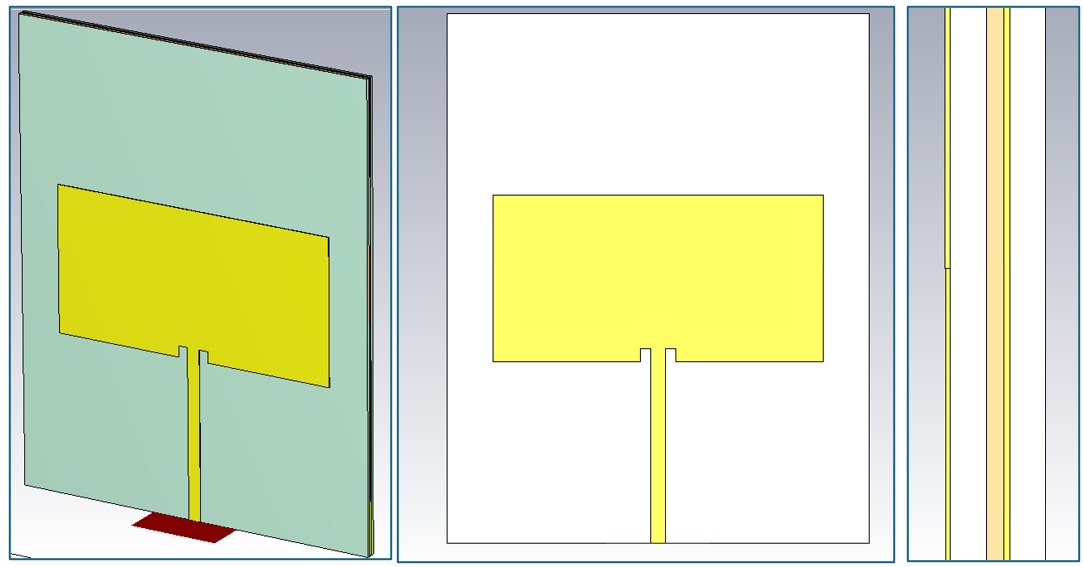
\includegraphics[width=0.5\linewidth]{Figures/chp3_CPW_patch_inset.png}
    \caption{Patch antenna model after designing the feed inset.}
    \label{fig:chp3_CPW_patch_inset}
    \end{figure}

\subsection{Masking the changing of the feed}
Referring to figure \ref{fig:chp3_incident_wave} in section \ref{sec:SysD} The reflected wave cannot be changed during operation, since it is determined by the physical structure of the reflector. The goal for this subsection is to minimize the phase difference caused by the reflected wave during the testing of different antennae. This allows to more accurately analyze the encoded phase of the re-radiated wave due to the changed termination of the reflector.

In the case of the reflector array the reflected wave’s magnitude decreases and the absorbed wave increases if the reflector is better matched. A perfect match is not practically realizable. For the test of the antenna the feed will change frequently with either an open circuit, 0$\Omega$ resistor or connector with a SMA 50$\Omega$ load connected to the feed. Figure \ref{fig:chp3_incident_wave_termination} below shows the possible placements for the feed termination. For figure \ref{fig:chp3_incident_wave_termination}(a) the reflected wave will change significantly as the feed termination is changed from open to short to matched.  For figure \ref{fig:chp3_incident_wave_termination}(b) the feed terminations will be masked by the antenna dielectric and the ground plane layer 3, refer to figure \ref{fig:chp3_stackup}. To achieve figure \ref{fig:chp3_incident_wave_termination}(b), an X-band via is required.

    \begin{figure}[H]
    \centering
    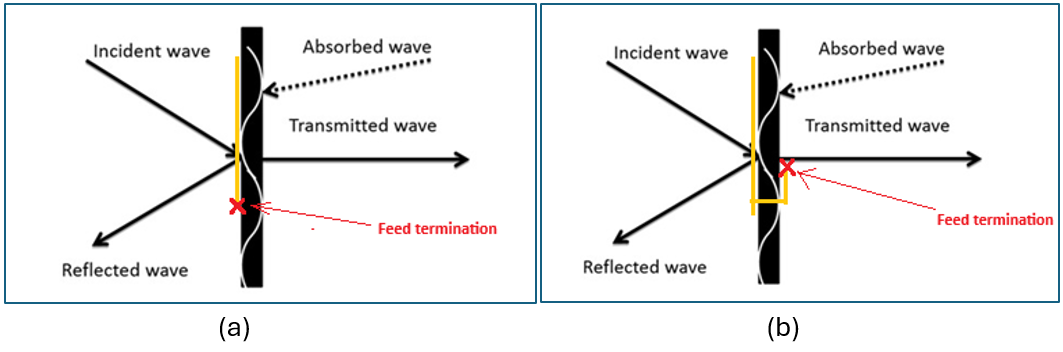
\includegraphics[width=0.7\linewidth]{Figures/chp3_incident_wave_termination.png}
    \caption{Possible placements of the terminations.}
    \label{fig:chp3_incident_wave_termination}
    \end{figure}

    \begin{figure}[H]
    \centering
    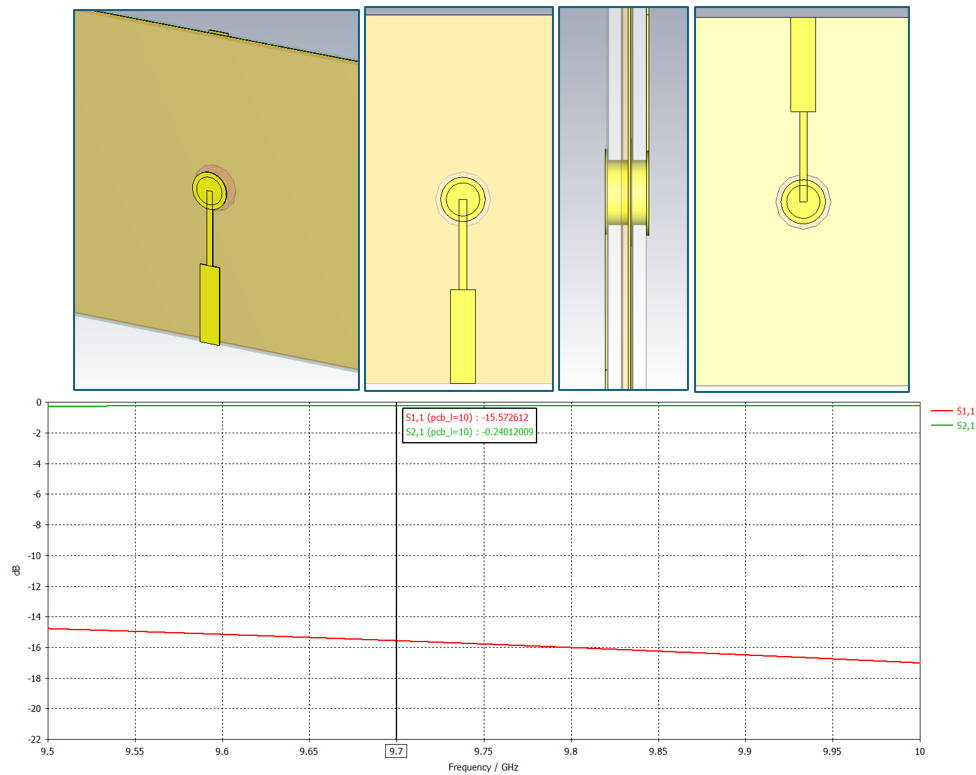
\includegraphics[width=0.85\linewidth]{Figures/chp3_CST_via_combined.png}
    \caption{X-band via and the frequency response.}
    \label{fig:chp3_CST_via_combined}
    \end{figure}

A X-band was designed previously for similar PCB stack-up. The via was simulated with the new stack-up to verify its performance. Figure \ref{fig:chp3_CST_via_combined} above show the via model simulated for the new stack-up along with its results. A return loss of 15.5dB and insertion loss of 0.24dB is seen at 9.7GHz. The via is added to the patch antenna. Figure \ref{fig:chp3_CPW_patch_via} below shows the final model for a single reflector array element. 

    \begin{figure}[H]
    \centering
    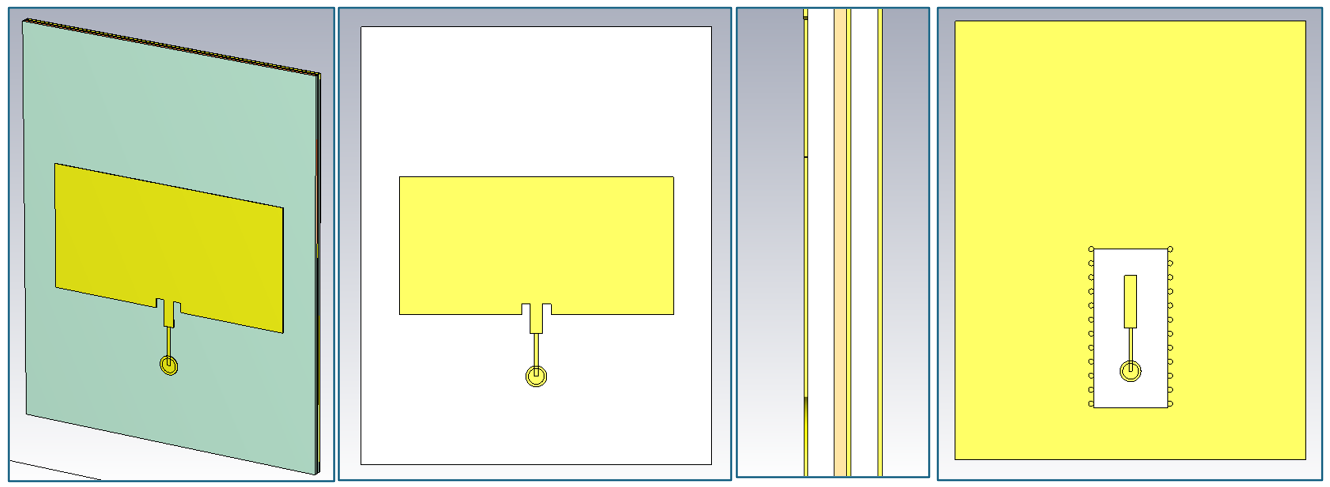
\includegraphics[width=0.6\linewidth]{Figures/chp3_CPW_patch_via.png}
    \caption{Final patch antenna model.}
    \label{fig:chp3_CPW_patch_via}
    \end{figure}

The bottom layer is designed to still be a microstrip trace, therefore the ground copper is pulled back more than twice the trace width. The distance between the edge of the 50$\Omega$ trace and the ground copper is equal to 1.76mm. The ground vias are blind vias to avoid changing the top layer of the antenna.

\subsection{Masking the changing of the feed}

    \begin{figure}[H]
    \centering
    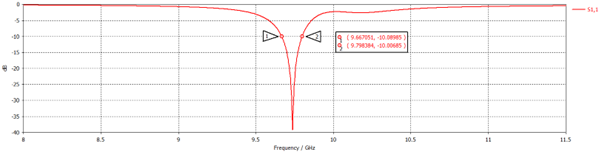
\includegraphics[width=0.99\linewidth]{Figures/chp3_CPW_patch_via_results.png}
    \caption{Simulated return loss of the final patch antenna in figure \ref{fig:chp3_CPW_patch_via}.}
    \label{fig:chp3_CPW_patch_via_results}
    \end{figure}

Figure \ref{fig:chp3_CPW_patch_via_results} above shows the return loss of the final antenna element that will be used for the testing in this report as well as in the reflector array for future testing. Figure \ref{fig:chp3_CPW_patch_via_results} show the final bandwidth (\(B_{-10dB}\)) is a 131MHz, which is close to the design goal of 150MHz. Figure \ref{fig:chp3_CPW_patch_via_pattern} below shows the Farfield pattern of the antenna, it is seen that the beamwidth is equal to 75°. The directivity is equal to 7.45dBi and no sidelobes are observed in the azimuth beam (Phi=0).

    \begin{figure}[H]
    \centering
    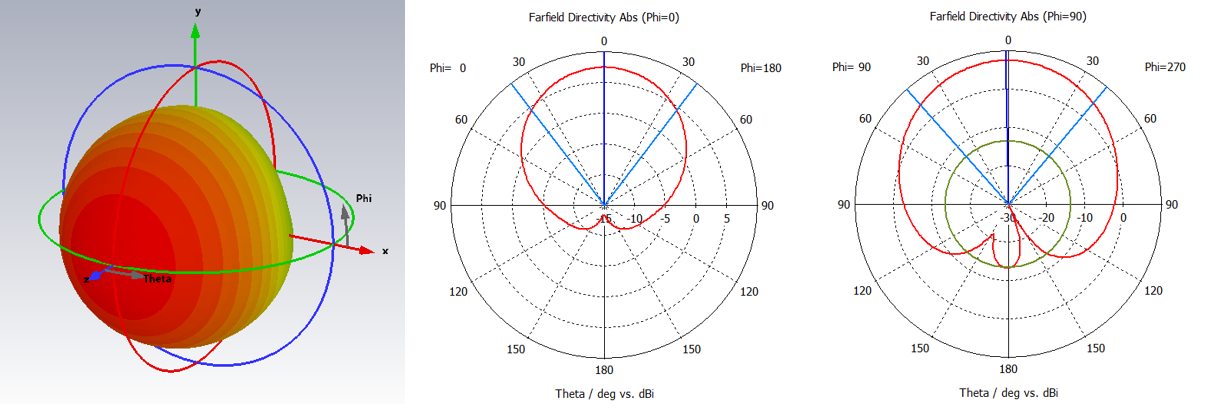
\includegraphics[width=0.9\linewidth]{Figures/chp3_CPW_patch_via_pattern.png}
    \caption{Simulated antenna pattern of the final patch antenna in figure \ref{fig:chp3_CPW_patch_via}.}
    \label{fig:chp3_CPW_patch_via_pattern}
    \end{figure}

Table \ref{tab:AntennaParam} below summarizes the antenna parameters including the parameters needed to manufacture the antenna. The Farfield distance of the antenna is calculated below with \(D=\max(L,\ W)\)
    \[R_{ff}=\frac{2D^2}{\lambda}=\frac{2{(15.65mm)}^2}{30.91mm}=15.85mm\]

    \begin{table}[H]
    \centering
    \caption{Dielectric comparison.}
    \begin{tabular}{|l|l|l|l|} 
    \hline
    \textbf{Parameter}  & \textbf{Symbol}   & \textbf{Value}    & \textbf{Unit}  \\ \hline
    Center Frequency    & \(f_0\)           & 9.70              & GHz            \\ \hline
    Wavelength          & \(\lambda\)       & 30.91             & mm             \\ \hline
    Dielectric Constant @ 9.7GHz&\(\epsilon_{r}\)& 3.78         & -              \\ \hline
    Substrate thickness & \(t\)             & 0.31              & mm             \\ \hline
    Patch length        & \(L\)             & 7.87              & mm             \\ \hline
    Bandwidth           & \(B_{-10dB}\)     & 131.33            & MHz            \\ \hline
    Patch width         & \(W\)             & 15.65             & mm             \\ \hline
    Patch ground length & \(L_g\)           & 25.00             & mm             \\ \hline
    Patch ground width  & \(W_g\)           & 20.00             & mm             \\ \hline
    copper thickness    & \(t_{cu}\)        & 35.00             & um             \\ \hline
    50 Ohm trace width  & \(W_{50\Omega}\)  & 0.68              & mm             \\ \hline
    Feed inset          & \(\Delta x_p\)    & 0.60              & mm             \\ \hline
    Feed gap            & \(\Delta g_p\)    & 0.50              & mm             \\ \hline
    Via hole diameter   & \(d_i\)           & 0.90              & mm             \\ \hline
    Via pad external pad diameter&\(d_p\)   & 0.60              & mm             \\ \hline
    Via ground pull back& \(d_o\)           & 1.50              & mm             \\ \hline
    Via matching strip width& \(W_strip\)   & 0.20              & mm             \\ \hline
    Via matching strip length measured from the center of the via & \(L_strip\)       
                                            & 2.45              & mm             \\
    \hline
    \end{tabular}
    \label{tab:AntennaParam}
    \end{table}

\subsection{Linear \& 2D reflector array design}
PCB manufacturers quote per dielectric sheet. Since a single element is only 25x20mm and this investigation only requires 3 antennas, a 1x4 and a 4x4 reflector were also designed for future testing and manufactured alongside the single elements.

Since the beam will not be steered the antenna spacing is not limited by a grating lobe requirement. This means the antennas can be spaced more than half a wavelength \(\left(\frac{\lambda}{2}\right)\). The antennas are space 20mm apart. This allows 4.35mm between the adjacent edges of the array elements. Figure \ref{fig:chp3_linear_array_combined} below shows the CST model along with the simulated coupling.

    \begin{figure}[H]
    \centering
    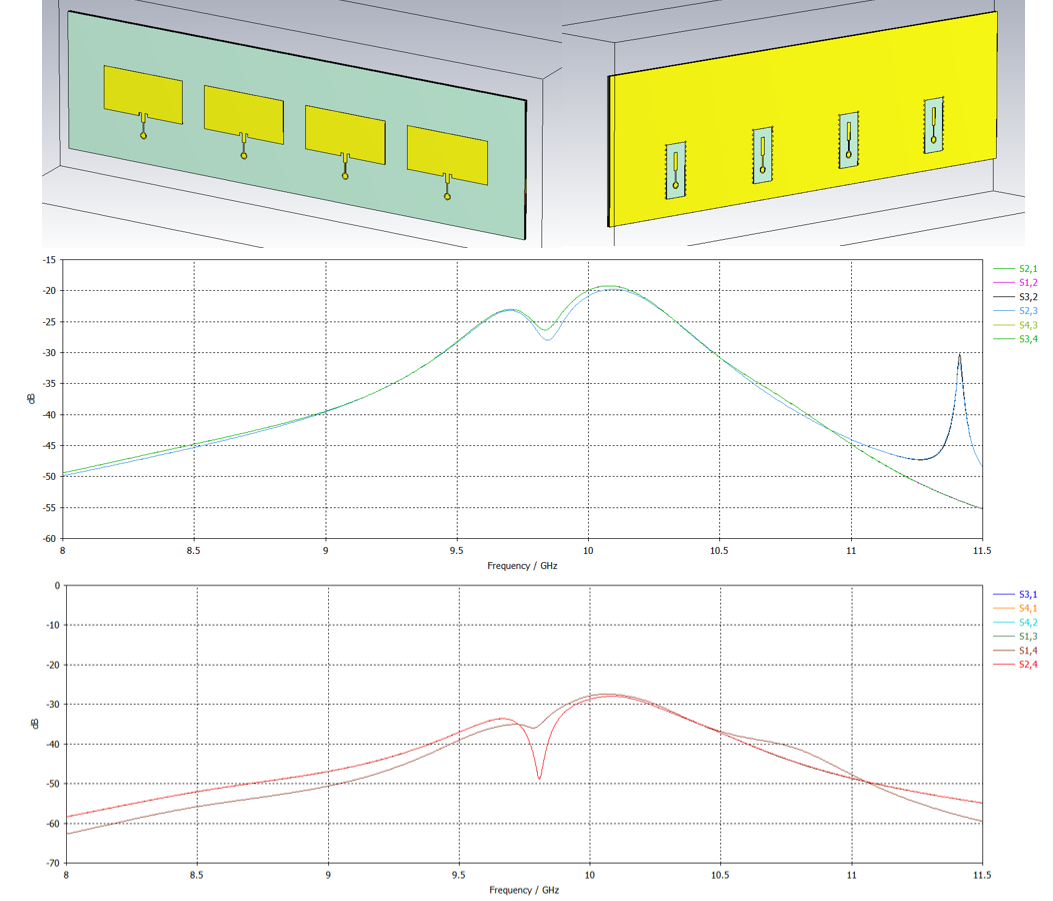
\includegraphics[width=0.99\linewidth]{Figures/chp3_linear_array_combined.png}
    \caption{Linear patch array and simulated coupling.}
    \label{fig:chp3_linear_array_combined}
    \end{figure}

Figure \ref{fig:chp3_linear_array_combined} graph shows the coupling from the adjacent array elements (top) and the coupling from every second element as well as the coupling between the edge elements (bottom). Figure ? below shows the return loss of all the elements. No variation is observed and the spacing is far enough that the coupling does not affect the antenna performance. The Farfield pattern is the Array Pattern (AP) times the Element Pattern (EP). Figure \ref{fig:chp3_linear_array_S11} below shows the Farfield pattern of the linear array, it is seen the beamwidth is equal to 19.5°. This is significantly lower than the 75° of a single element due to the array pattern having a narrow beamwidth. The gain of the array is equal to 13.17dBi, which is a 5.72dB improvement from the single element. A Sidelobe level (SLL) of -13.2dBc or -0.03dBi is observed.
    \[AP*EP=Farfield\ Pattern\]

    \begin{figure}[H]
    \centering
    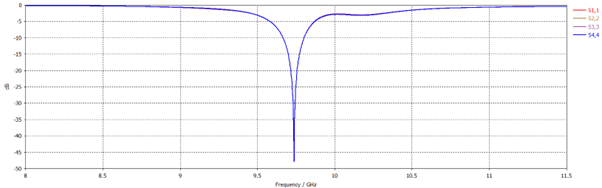
\includegraphics[width=0.99\linewidth]{Figures/chp3_linear_array_S11.png}
    \caption{Simulated return loss of the linear patch array.}
    \label{fig:chp3_linear_array_S11}
    \end{figure}

    \begin{figure}[H]
    \centering
    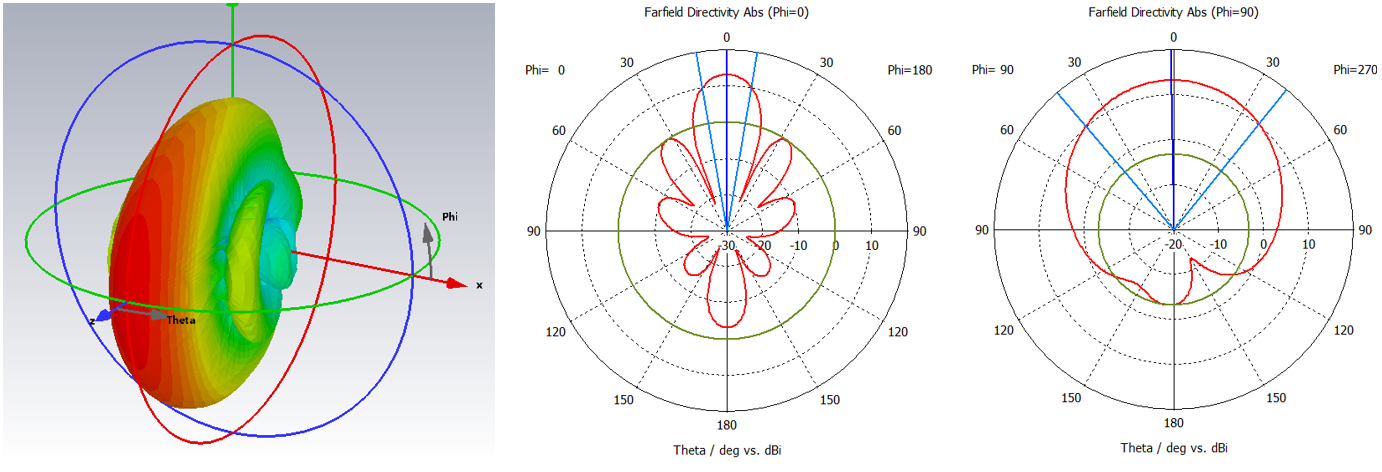
\includegraphics[width=0.8\linewidth]{Figures/chp3_linear_array_pattern.png}
    \caption{Simulated farfield pattern of the linear patch array.}
    \label{fig:chp3_linear_array_pattern}
    \end{figure}

The linear array was adapted to a 2-dimensional reflector array with the vertical antenna spacing also equal to 20mm. This allows 8mm between the top edge of the array elements and the edge of the via pad. Figure \ref{fig:chp3_2D_array_combined} below shows the CST model along with the simulated coupling. 

    \begin{figure}[H]
    \centering
    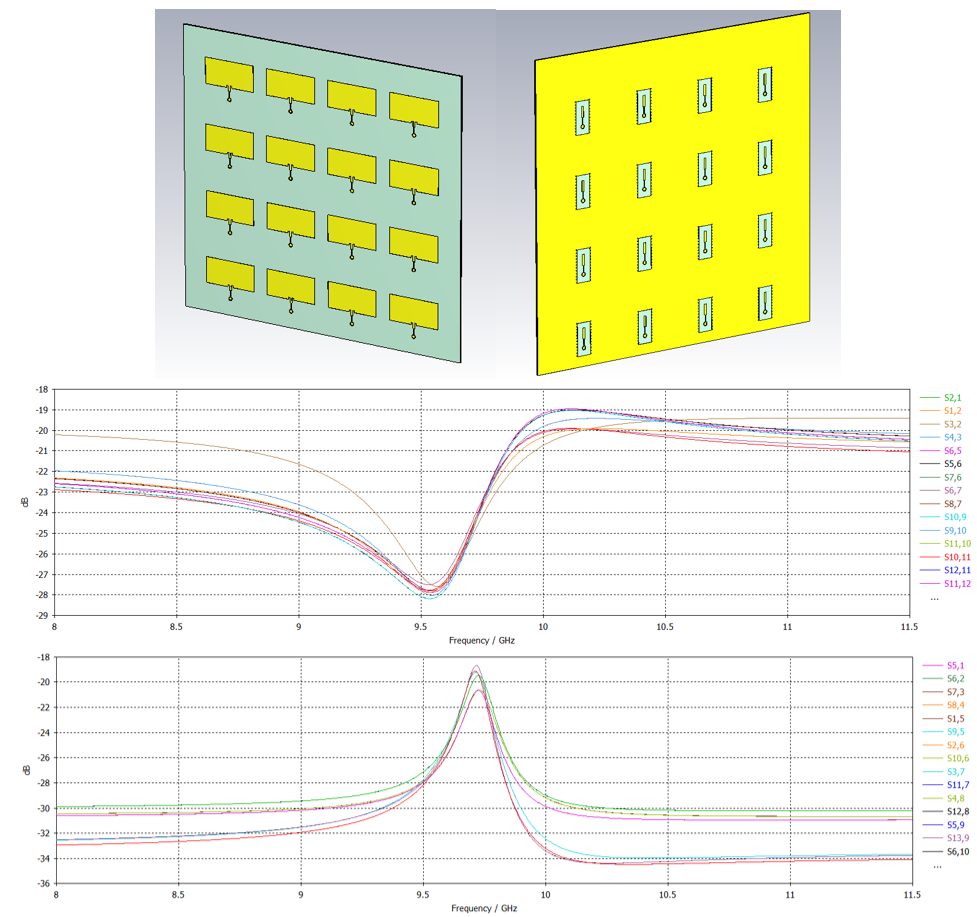
\includegraphics[width=0.99\linewidth]{Figures/chp3_2D_array_combined.png}
    \caption{2D patch array and simulated coupling.}
    \label{fig:chp3_2D_array_combined}
    \end{figure}

Figure \ref{fig:chp3_2D_array_combined} shows the coupling from the horizontally adjacent array elements (top) and the coupling from the vertically adjacent array elements (bottom). Figure \ref{fig:chp3_2D_array_S11} below shows the return loss of all the elements. No variation is observed and the spacing is far enough that the coupling does not affect the antenna performance. Figure \ref{fig:chp3_2D_array_pattern} below shows the Farfield pattern of the 2-dimensional array, it is seen the beamwidth is equal to 19.4°. The gain of the array is equal to 13.14dBi, which very similar to the linear array. The sidelobe level (SLL) of -14.3dBc or -0.26dBi is observed, which is a 1dB improvement over the linear array.

    \begin{figure}[H]
    \centering
    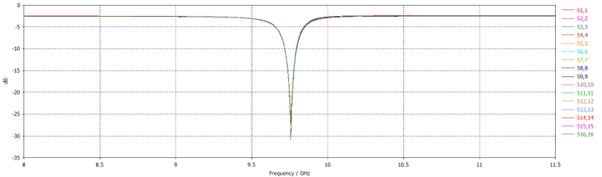
\includegraphics[width=0.99\linewidth]{Figures/chp3_2D_array_S11.png}
    \caption{Simulated return loss of the 2D patch array.}
    \label{fig:chp3_2D_array_S11}
    \end{figure}

    \begin{figure}[H]
    \centering
    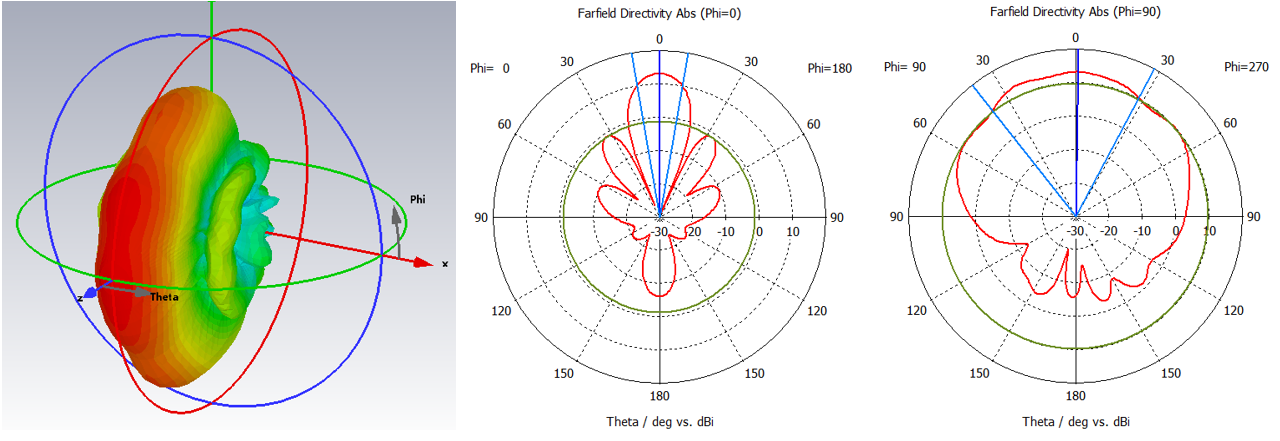
\includegraphics[width=0.7\linewidth]{Figures/chp3_2D_array_pattern.png}
    \caption{Simulated farfield pattern of the 2D patch array.}
    \label{fig:chp3_2D_array_pattern}
    \end{figure}

\subsection{Manufacturing}

    \begin{figure}[H]
    \centering
    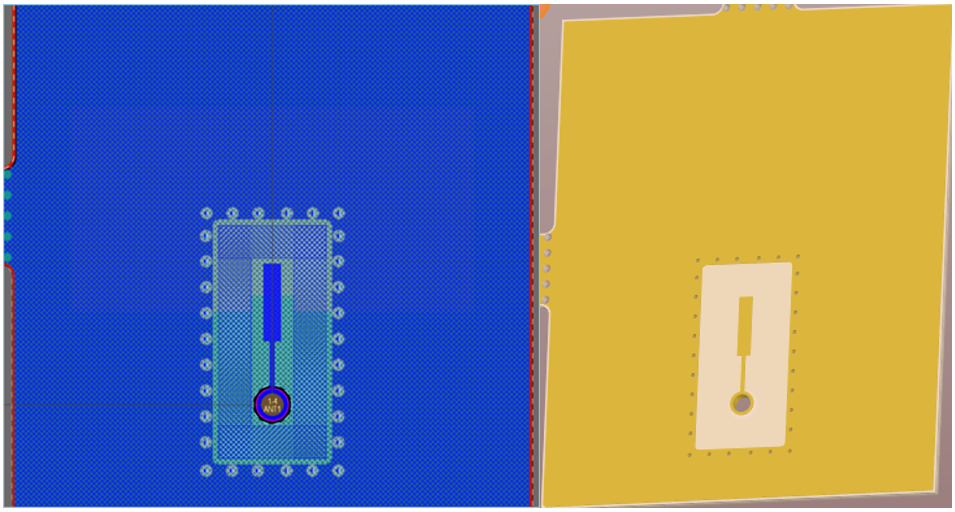
\includegraphics[width=0.5\linewidth]{Figures/chp3_Altium_single.png}
    \caption{Single patch antenna in Altium.}
    \label{fig:chp3_Altium_single}
    \end{figure}

To be able to measure the response of the antenna, a connector is required. Figure \ref{fig:chp3_Altium_single_SMP} below shows the Altium 2D and 3D view of the surface mount SMP connector used. Since the interest is focussed on the open and short circuit termination the effort of designing the RF transition was not done, the manufacturers recommended footprint up to 18GHz is used.

    \begin{figure}[H]
    \centering
    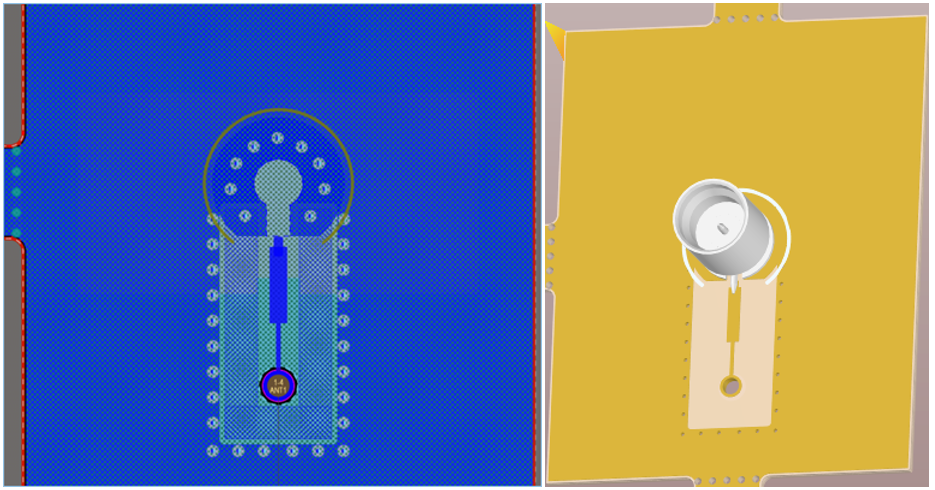
\includegraphics[width=0.5\linewidth]{Figures/chp3_Altium_single_SMP.png}
    \caption{Single patch antenna with a SMP connetor in Altium.}
    \label{fig:chp3_Altium_single_SMP}
    \end{figure}

Maximizing the use of the dielectric sheet size as specified by the PCB manufacturer results in the final PCB seen in figure \ref{fig:chp3_Altium_all} below. Four single antenna elements are manufactured, two of which as a SMP connector on the feed. One of the two single elements without a connector will remain an open circuit, whilst the other element will be shorted with a 0$\Omega$ resistor.

    \begin{figure}[H]
    \centering
    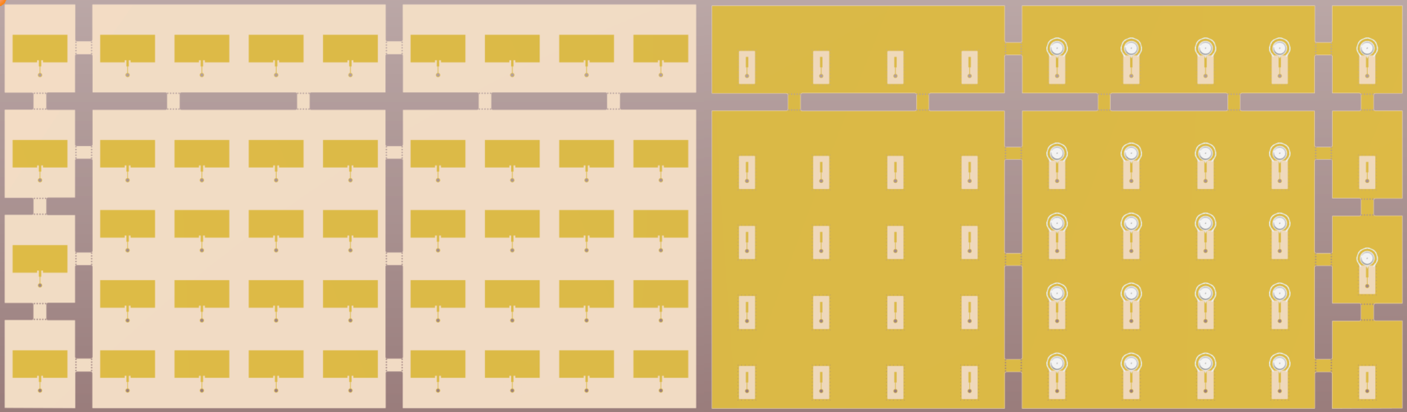
\includegraphics[width=0.8\linewidth]{Figures/chp3_Altium_all.png}
    \caption{Manufactured Altium PCB.}
    \label{fig:chp3_Altium_all}
    \end{figure}

The manufactured antenna has a visible warp and due to this a mounting solution is required that will pull the antenna flat again. The warping is due to the very thin PCB thickness of 624um and the removed copper on layer 2 creating an asymmetrical stack-up. A better antenna design would include mounting hole to screw the antenna to a plate or bracket.

    \begin{figure}[H]
    \centering
    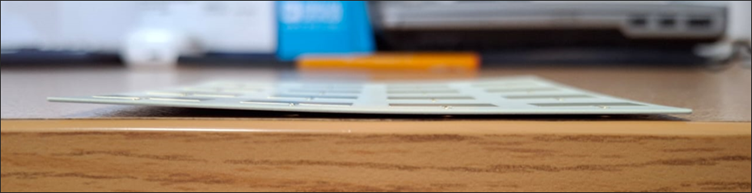
\includegraphics[width=0.8\linewidth]{Figures/chp3_physical_warp.png}
    \caption{Manufactured patch array with visible warping.}
    \label{fig:chp3_physical_warp}
    \end{figure}

The quickest solution available due to the lack of mounting holes was a 3D printed bracket. The first solution below securely held the antenna in place with no visible flexing or cracking.

    \begin{figure}[H]
    \centering
    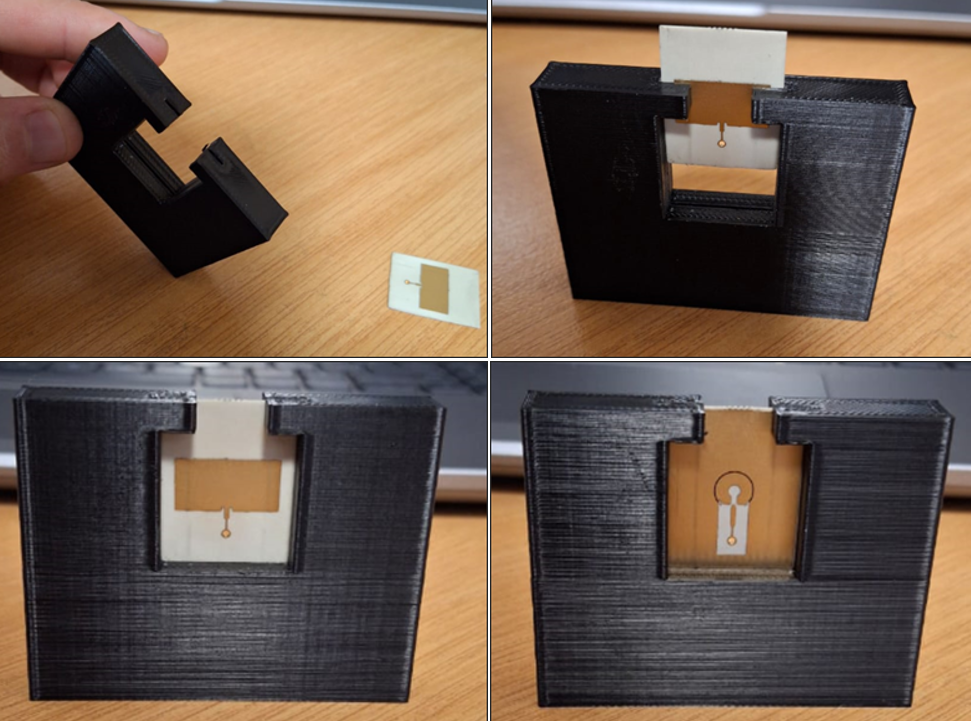
\includegraphics[width=0.4\linewidth]{Figures/chp3_failed_bracket.png}
    \caption{First iteration of the mounting bracket.}
    \label{fig:chp3_failed_bracket}
    \end{figure}
    
However, the bracket was not high enough to easily align the three antennae using during testing. Also, due to the wide beamwidth of a single element patch antenna there was still a concern the 90◦ edges left and right of the antenna are seen by the beam.

    \begin{figure}[H]
    \centering
    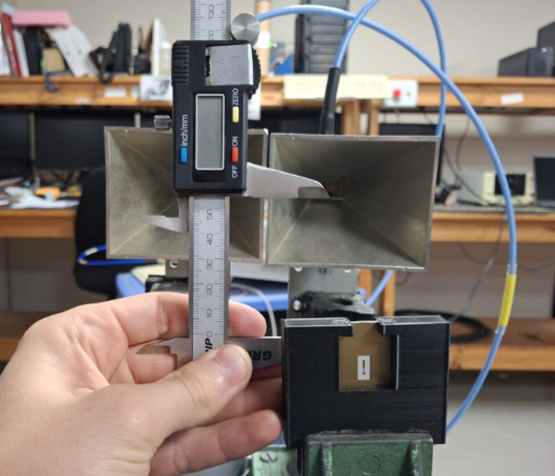
\includegraphics[width=0.3\linewidth]{Figures/chp3_failed_bracket_height.png}
    \caption{Height misalignment of the first bracket.}
    \label{fig:chp3_failed_bracket_height}
    \end{figure}

The second version solve both issues by increasing the height of the bracket as well as adding 45◦ chamfers to the front face of the bracket.

    \begin{figure}[H]
    \centering
    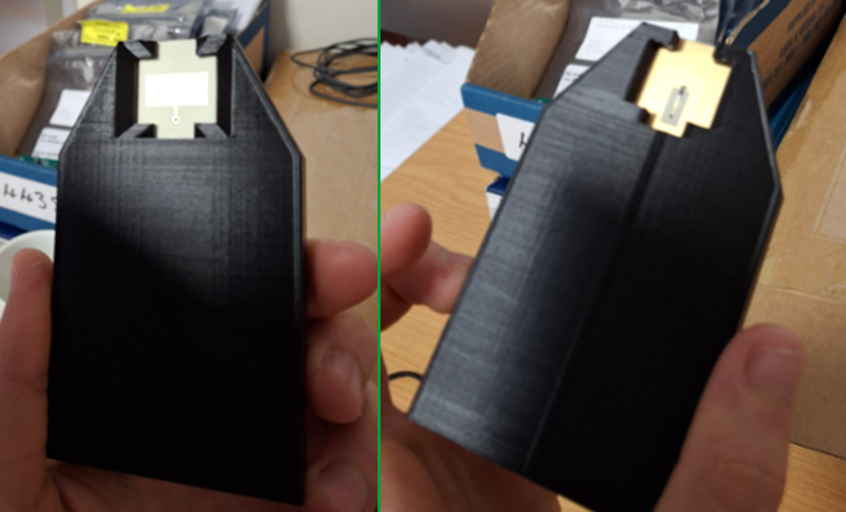
\includegraphics[width=0.4\linewidth]{Figures/chp3_bracket.png}
    \caption{First iteration of the mounting bracket.}
    \label{fig:chp3_bracket}
    \end{figure}

\section{Measurement Processing}

    \begin{figure}[H]
    \centering
    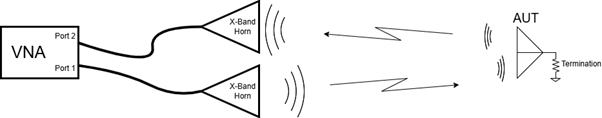
\includegraphics[width=0.8\linewidth]{Figures/chp3_setup.png}
    \caption{Block diagram of the required test setup.}
    \label{fig:chp3_setup}
    \end{figure}

Figure \ref{fig:chp3_setup} shows the planned test setup. A two port Vector Network Analyzer (VNA) is required to be able to measure the phase of the received reflected signals from the Antenna Under Test (AUT). Unfortunately the VNA will measure more than just the re-radiated signal from the reflector and the measured  \(S_{21}\) parameter will need to be processed to isolate the phase encoded signal. 

    \begin{figure}[H]
    \centering
    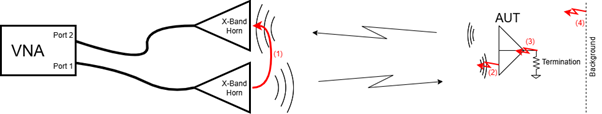
\includegraphics[width=0.8\linewidth]{Figures/chp3_setup_reflections.png}
    \caption{Reflections measured by the receiver horn antenna.}
    \label{fig:chp3_setup_reflections}
    \end{figure}
    
Referring to figure \ref{fig:chp3_setup_reflections} above, the received signal at port 2 will be the superposition the following:
\begin{enumerate}
    \item The coupled signal from transmitter X-Band horn antenna.
    \item The reflected signal from the antenna, refer to figure \ref{fig:chp3_incident_wave} in section \ref{sec:SysD}.
    \item The re-radiated signal, which will be encoded with a phase.
    \item The reflected signals from the surrounding background.
\end{enumerate}

For the proposed system in section \ref{sec:objectives} to be realizable, the effect of signals (1), (2) and (4) needs to be able to be calibrated out of the received signal at port 2. The same applies to the tests required for this investigation. To solve this a 50$\Omega$ load is connected to the antenna for a separate matched measurement. The assumption is that if all of the absorbed wave from the AUT is also absorbed by the matched load connected to the antenna, then the signal measured at port 2 will only consist of signals (1), (2) and (4). Therefore, if the \(S_{21}\) of the matched measurement is subtracted from the \(S_{21}\) at of the open and short circuit measurement, the only remaining signal is (2), the re-radiated signal, which will be encoded with a phase.

The processing chain to achieve is described in this section. The processing chain is written in MATLAB after saving the touchstone files from the VNA. The script opens and reads only the \(S_{21}\) from the required touchstone files. The \(S_{21}\) of the matched, open and short circuit measurement are plotted on a smith chart at the center frequency of 9.7GHz. The matched \(S_{21}\) is then subtracted from the open and short circuit measurement and plotted again to verify.

    \begin{figure}[H]
    \centering
    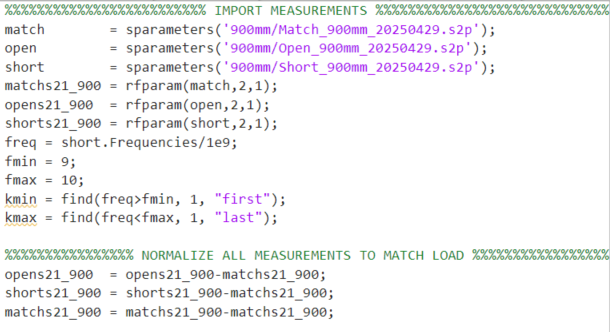
\includegraphics[width=0.6\linewidth]{Figures/chp3_code_import_norm.png}
    \caption{MATLAB script to import and normalize the \(S_{21}\) to the 50$\Omega$ \(S_{21}\).}
    \label{fig:chp3_code_import_norm}
    \end{figure}


As stated in section \ref{sec:OCSO50} the signal at a short circuit will be reflected with a 180° phase change, but the signal at an open circuit will be reflected with no phase change. Therefore, the theoretical phase between the open and the short circuit measurement after subtracting the matched measurement should be a fixed 180° difference. The script therefore subtracts the phase of the short circuit measurement from the open circuit measurement and plots the results over frequency. All the samples in the bandwidth of the antenna is then used to calculate the mean and the standard deviation of phase difference. The error is then measured from the mean for all measurements that were imported.

    \begin{figure}[H]
    \centering
    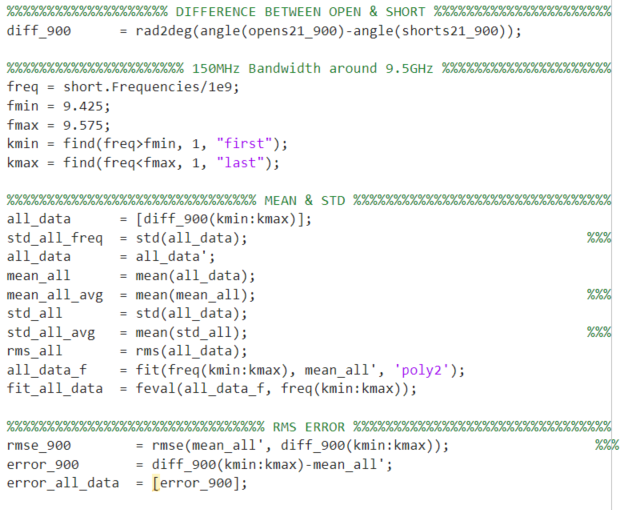
\includegraphics[width=0.6\linewidth]{Figures/chp3_code_diff_stats.png}
    \caption{MATLAB script to analyze the encoded phase and the error of the AUT.}
    \label{fig:chp3_code_diff_stats}
    \end{figure}

It is crucial to only subtract the phases of each \(S_{21}\) and not the complex values. If the complex value is subtracted first then the resulting phase would be \(\Phi\) in figure \ref{fig:chp3_smithchart_vector} below and not \(\Theta\).

    \begin{figure}[H]
    \centering
    \includegraphics[width=0.4\linewidth]{Figures/chp3_smithchart_vector.png}
    \caption{Smith chart with phase relative phase angles.}
    \label{fig:chp3_smithchart_vector}
    \end{figure}

% ----------------------------------------------------
\ifstandalone
\bibliography{../Bibliography/References.bib}
\printnoidxglossary[type=\acronymtype,nonumberlist]
\fi
%\end{document}
% ----------------------------------------------------